\documentclass[11pt]{article}
\usepackage{geometry}                % See geometry.pdf to learn the layout options. There are lots.
\geometry{a4paper}                   % ... or a4paper or a5paper or ... 
\usepackage{graphicx}
\usepackage{amssymb}
\usepackage{url}
\usepackage{listings}
\usepackage{color}

\renewcommand{\textfraction}{0.15}
\renewcommand{\topfraction}{0.85}
\renewcommand{\bottomfraction}{0.65}
\renewcommand{\floatpagefraction}{0.60}

\usepackage{fontspec,xltxtra,xunicode}
\defaultfontfeatures{Mapping=tex-text}
\setromanfont[Mapping=tex-text]{Georgia}
\setsansfont[Scale=MatchLowercase,Mapping=tex-text]{Tahoma}
\setmonofont[Scale=MatchLowercase]{Courier New}


\title{IEG4180 Project 1\\NetProbe Report}
\author{GUAN Hao\\05569511\\hguan5@ie.cuhk.edu.hk}
\date{\today}
\begin{document}
\maketitle
\section{Experiment and Result}
\subsection{Using TCP}
According to the project specification, I did the experiment by using my own program. The experiment results is shown below.

\begin{figure}
\centering
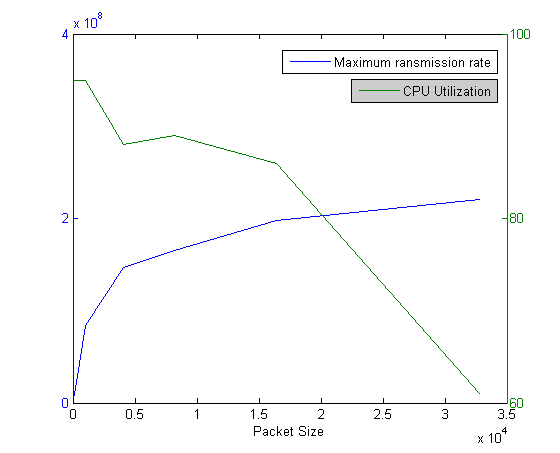
\includegraphics[width=3in]{TCP.png}
\caption{TCP experiment result plot.}
\label{fig:TCP}
\end{figure}
When using TCP protocol, the maximum transmission rate increases as the packet size raises. However the the CPU utilization becomes lower when the packet size is larger. Therefore, the program has high performance if a large packet size is chosen.

\subsection{Using UDP}
\begin{figure}
\begin{minipage}[c]{0.5\textwidth} 
\centering 
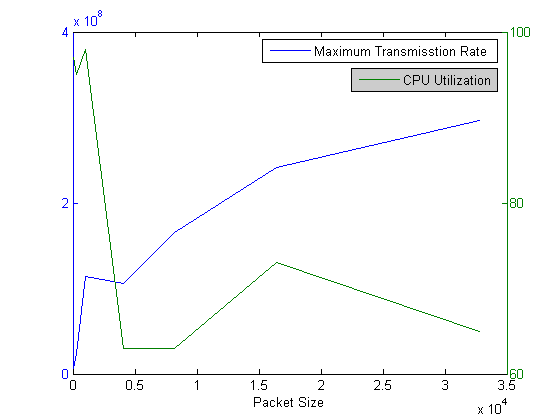
\includegraphics[width=3in]{UDP1.png} 
\end{minipage}% 
\begin{minipage}[c]{0.5\textwidth} 
\centering 
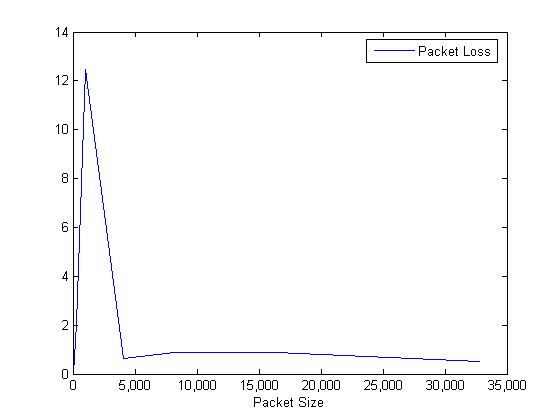
\includegraphics[width=3in]{UDP2.png}
\end{minipage}% 
\caption{TCP experiment result plot.}
\label{fig:TCP}
\end{figure}
When using UDP protocol, the maximum transmission rate and CPU utilization has the similar trend as using TCP. However, UDP can reach higher speed if the same packet size is chosen. Because UDP is not reliable, packet loss is also a very important value in this experiment. The figure of packet loss is interesting: it seems to be a normal distribution shape. The packet loss is very high when the packet size is 1,024 bytes however it can be very low if the packet size is small or very large.

\appendix
\section{Data}
%\begin{table}
\subsection{TCP}
\begin{center}
\begin{tabular}{ccc}
Packet Size(Byte) & Max Transmission Rate(Bps) & CPU Utilization(\%) \\ [0.5ex]
\hline\hline
64	& 5139760  & 95 \\
256 & 21746966 & 95 \\
1024 & 84000487 & 95 \\
4096 & 147170336 & 88 \\
8192 & 164837112 & 89 \\
16384 & 198248687 & 86 \\ 
32768 & 220174930 & 61 \\
\hline
\end{tabular}
\end{center}


\subsection{UDP}
\begin{center}
\begin{tabular}{cccc}
Packet Size(Byte) & Max Transmission Rate(Bps) & CPU Utilization(\%) & Packet Loss\\ [0.5ex]
\hline\hline
64	& 6712258 & 97 & 0.03 \\
256 & 23943618 & 95 & 2.07 \\
1024 & 113792498 & 98 & 12.46 \\
4096 & 106087247 & 63 & 0.65 \\
8192 & 165729706 & 63 & 0.87 \\
16384 & 241019130 & 73 & 0.87 \\
32768 & 296052042 & 65 & 0.52 \\
\hline
\end{tabular}
\end{center}
\section{Declaration}
I declare that the assignment here submitted is original except for source material explicitly acknowledged, and that the same or related material has not been previously submitted for another course. I also acknowledge that I am aware of University policy and regulations on honesty in academic work, and of the disciplinary guidelines and procedures applicable to breaches of such policy and regulations, as contained in the website \url{http://www.cuhk.edu.hk/policy/academichonesty/}
\end{document}
